\subsection{3 Phasen 400 V 50 Hz Netz}
\begin{minipage}{0.4 \linewidth}
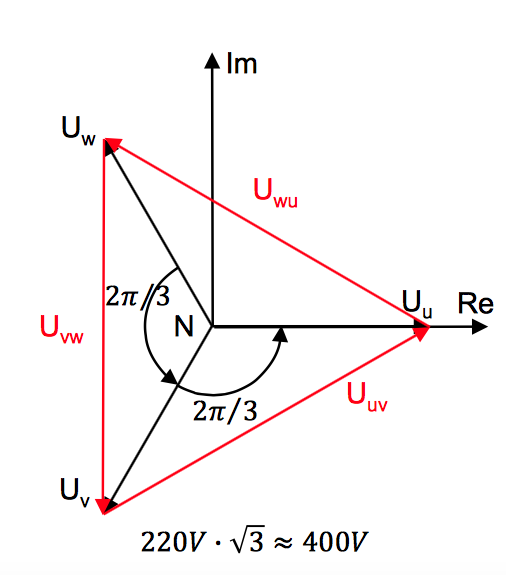
\includegraphics[width = 0.8 \linewidth]{./Pics/VL89/Drehstrom}
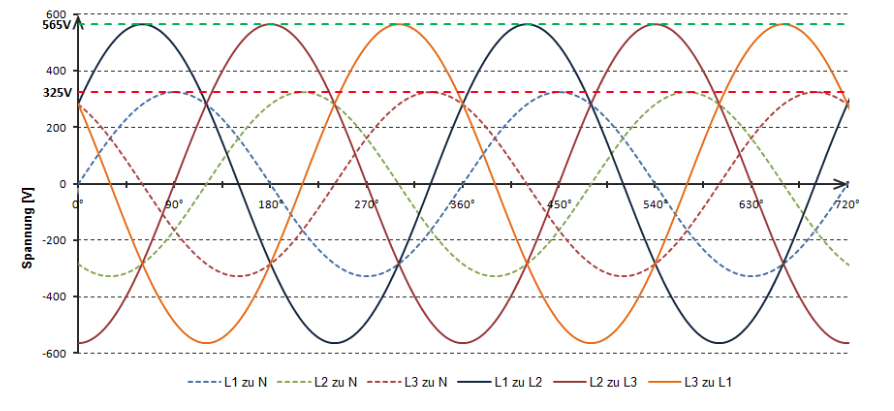
\includegraphics[width = \linewidth]{./Pics/VL89/Drehstrom2}
\end{minipage}
\begin{minipage}{0.6 \linewidth}
Das öffentliche 400-V-Drehstromnetz basiert auf drei $120^\circ$ zeitversetzten sinusförmigen Spannungen: 

$u_U(t) = U_m \cdot sin(\omega t)$ \\

$u_V(t) = U_m \cdot sin(\omega t - 2\pi/3)$ \\

$u_W(t) = U_m \cdot sin(\omega t - 4\pi/3)$ \\

Die Sternspannungen sind die Spannungen zwischen dem Neutralleiter und einem Aussenleiter: \\

$U_U, U_V,U_W$ \\

Die verketteten Spannungen sind die Spannungen zwischen den Aussenleitern:

$U_{UV}, U_{VW},U_{WU}$ \\

Die Spannungen von Dreiphasensystemen werden gemäss DIN 40108 nach dem Effektivwert der verketteten Spannung benannt, für die in Europa üblichen Niederspannungsnetzte beispielsweise als 400-V-Drehstromnetz.
\end{minipage}

\subsection{Erzeugung eines magnetischen Drehfelds}
\begin{minipage}{0.5 \linewidth}
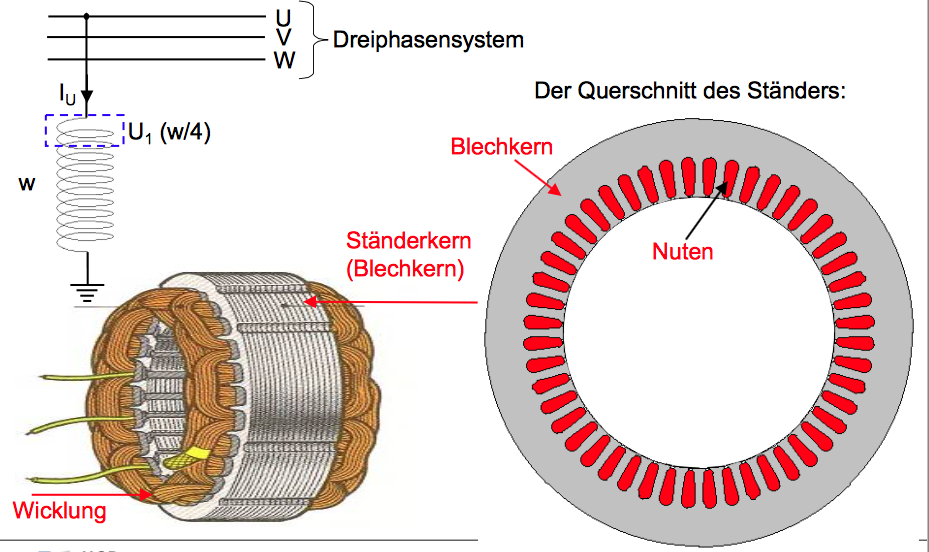
\includegraphics[width = \linewidth]{./Pics/VL89/Drehfeld}
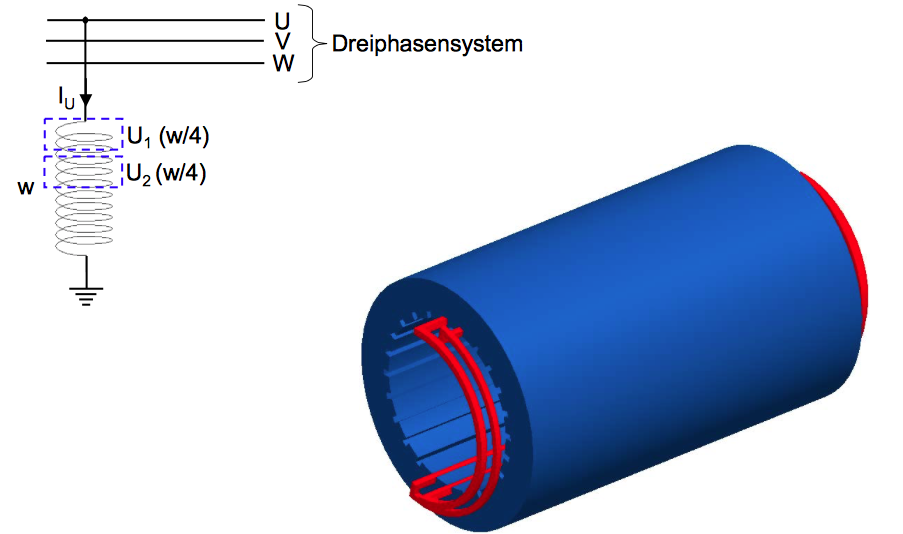
\includegraphics[width = \linewidth]{./Pics/VL89/Drehfeld3}
\end{minipage}
\begin{minipage}{0.5 \linewidth}
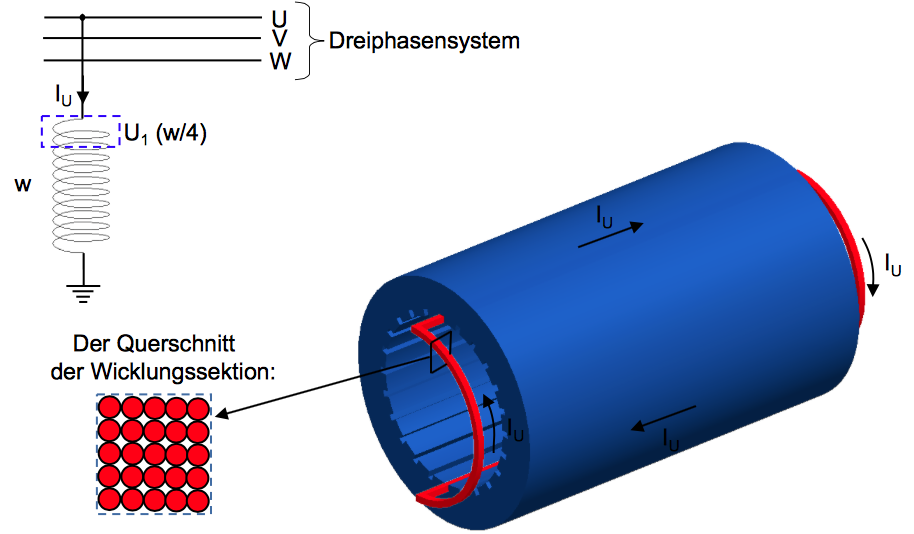
\includegraphics[width = \linewidth]{./Pics/VL89/Drehfeld2}
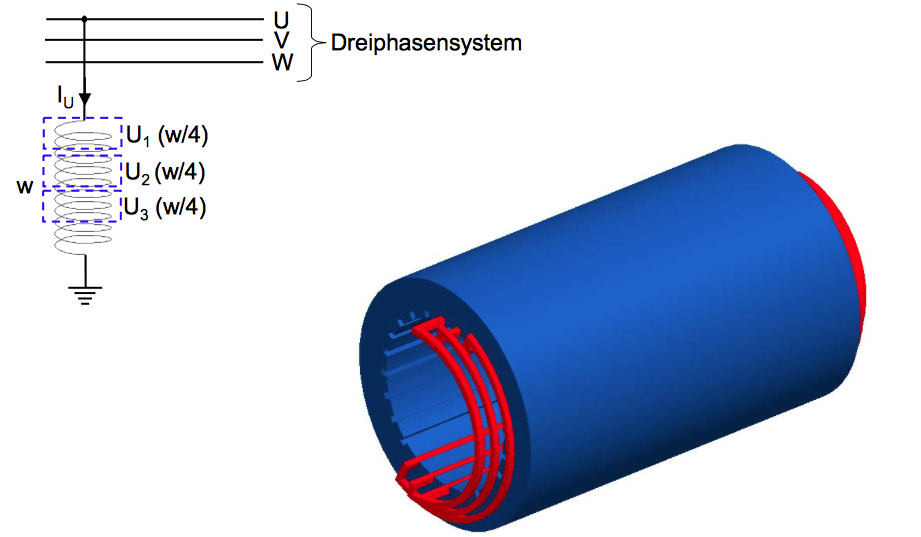
\includegraphics[width = \linewidth]{./Pics/VL89/Drehfeld4}
\end{minipage}

\begin{minipage}{0.5 \linewidth}
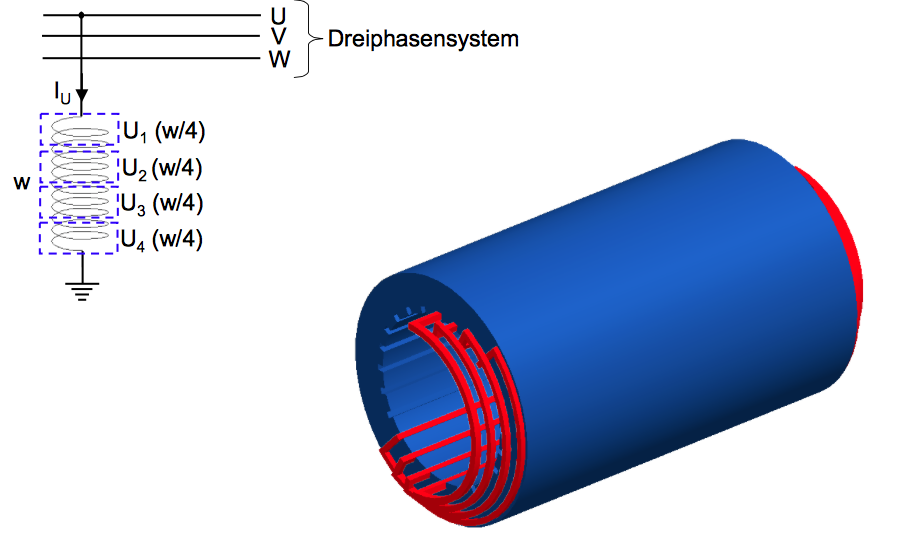
\includegraphics[width = \linewidth]{./Pics/VL89/Drehfeld5}
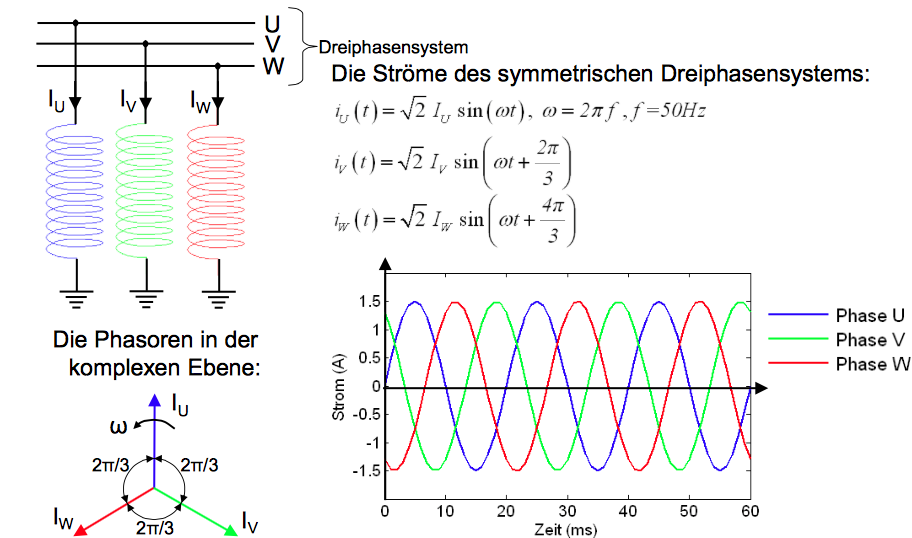
\includegraphics[width = \linewidth]{./Pics/VL89/Drehfeld7}
\end{minipage}
\begin{minipage}{0.5 \linewidth}
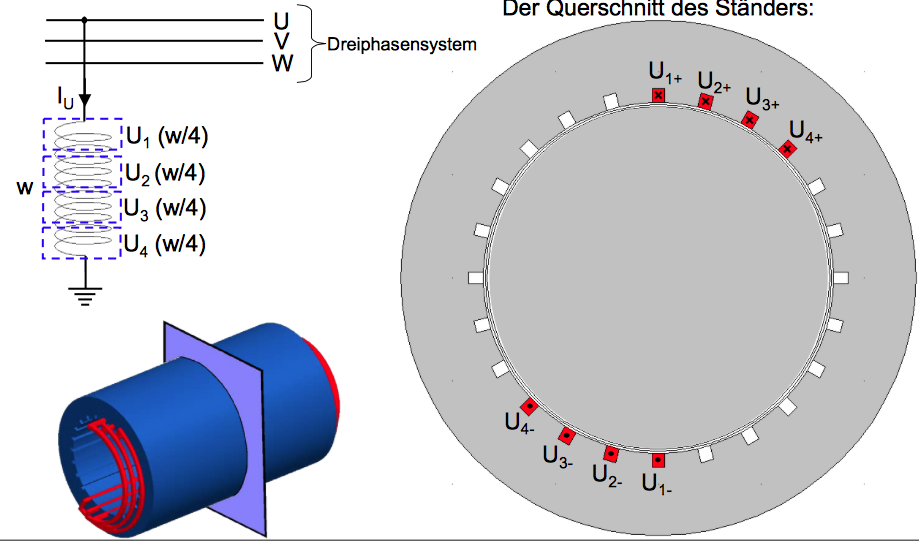
\includegraphics[width = \linewidth]{./Pics/VL89/Drehfeld6}
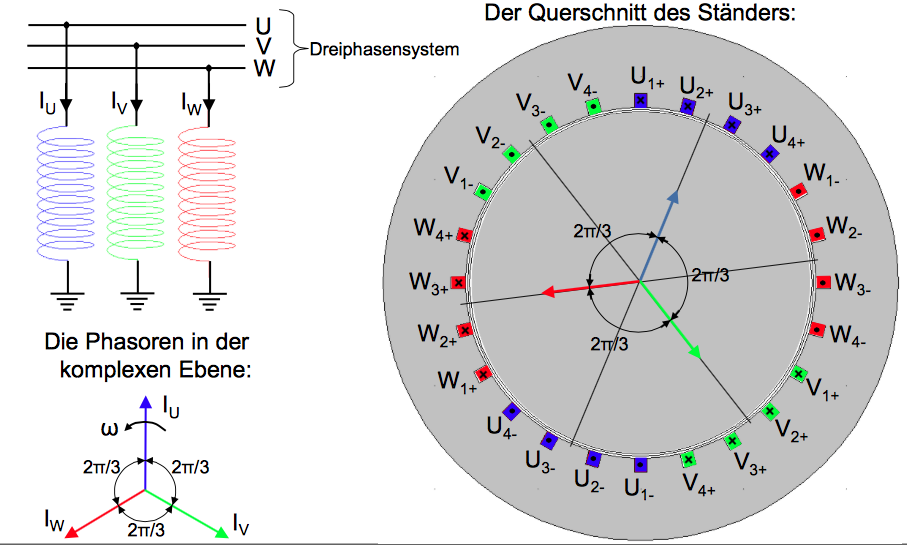
\includegraphics[width = \linewidth]{./Pics/VL89/Drehfeld8}
\end{minipage}

\subsection{Grundbegriffe}


\begin{minipage}{0.3 \linewidth}
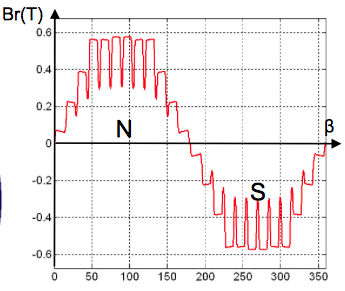
\includegraphics[width = \linewidth]{./Pics/VL89/Grundbegriff}
\end{minipage}
\begin{minipage}{0.7 \linewidth}
\begin{itemize}
\item Polpaarzahl: p =1
\item Polzahl 2p = 2
\item Nutzahl: N =24
\item Nutzahl pro Phasenband q = 4
\item N = $2p \cdot q \cdot m$
\item Strangzahl: m = 3
\item Läuferumfang: $\beta$ = [0, 360]
\item Drehzahl: n = $frac{60 \cdot f}{p}$ $min^{-1}$ 
\end{itemize}
\end{minipage}

\begin{minipage}{0.5 \linewidth}
\centering
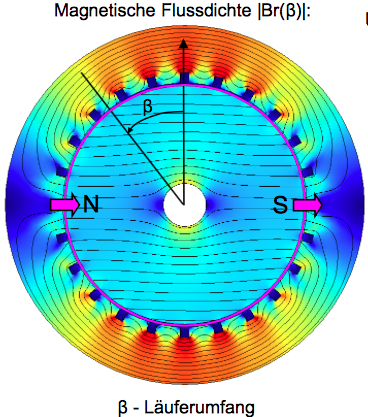
\includegraphics[width = 0.5 \linewidth]{./Pics/VL89/Grundbegriff2}
\end{minipage}
\begin{minipage}{0.5 \linewidth}
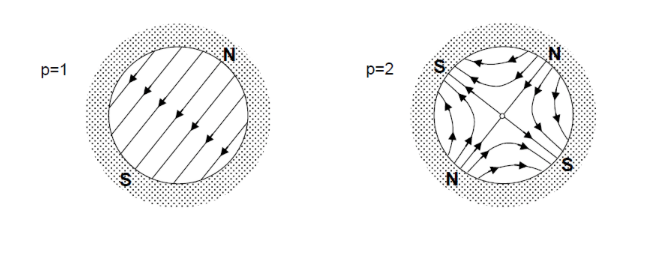
\includegraphics[width = \linewidth]{./Pics/VL89/Polpaar}
\end{minipage}

\begin{minipage}{0.5 \linewidth}
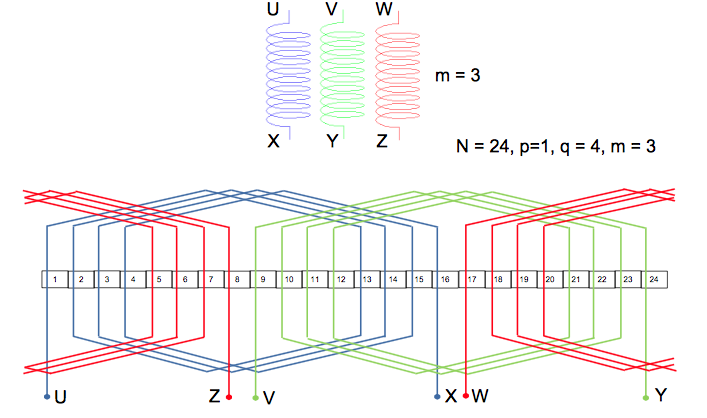
\includegraphics[width = \linewidth]{./Pics/VL89/Wicklungsschema}
\end{minipage}

